% ==============================================================================
\chapter{Timepix3 telescope performance}
\label{ch:Timepix3Telescope}
%==============================================================================    

\section{AllPix: a \textsc{Geant4}-based simulation software}
AllPix~\cite{allpix}, is used as a wrapper on \textsc{Geant4} to
simulate the test beam setup. The software is written in C/C++. It
provides a flexible interface to define the geometry of the
setup. \cref{fig:TPX3TelescopeAllpix} shows the telescope planes
and the DUT simulated in AllPix.

\begin{figure}[htbp]
  \centering
  \begin{tikzpicture}
    \node[anchor=south west,inner sep=0] (image) at
    (0,0){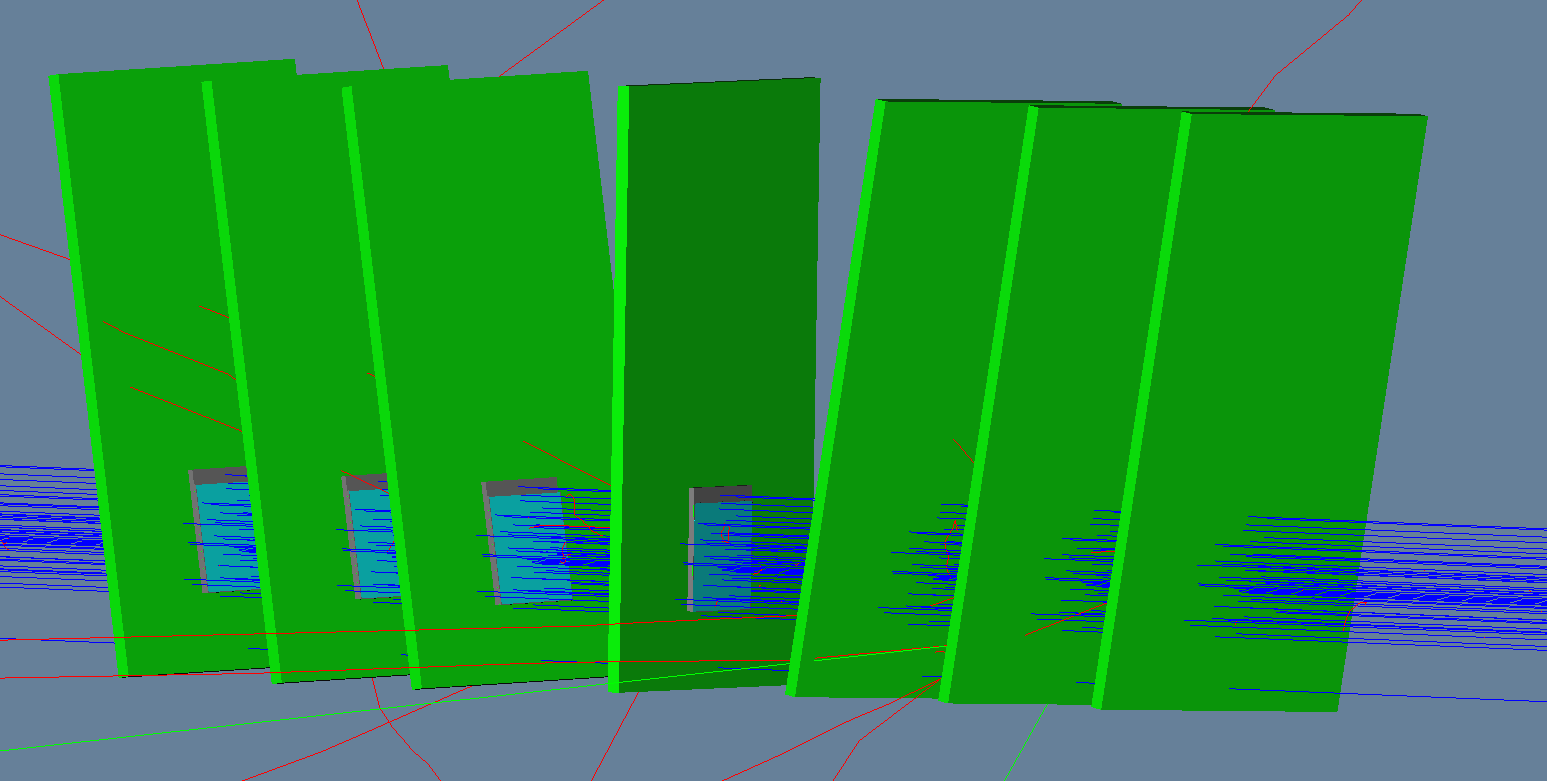
\includegraphics[width=0.8\textwidth]{figures/ActiveEdge/Allpix_telescope_withParticles.png}};
    \begin{scope}[x={(image.south east)},y={(image.north west)}]
      \node[above, color=white] at (0.45, 0.65) {\textbf{DUT}};
    \end{scope}
  \end{tikzpicture}
  \caption{Simulation of the Timepix3 telescope with AllPix.}
  \label{fig:TPX3TelescopeAllpix}
\end{figure}

The main components of the software are described here-below:
\begin{enumerate}
\item Digitiser: \textsc{Geant4}, for each simulation step
  (\texttt{G4Step}) through the matter, provides the energy deposited
  in the sensitive material. The step length can be customised. For
  thin sensors simulations a step of $2\,\micron$ is selected and
  provides a precise energy deposition. The semiconductor physics in a
  Silicon detector is then defined in the digitiser. The drift and
  diffusion are performed at each step to simulate the electron-hole
  pair movement in the electric and magnetic fields. The readout ASIC
  is also simulated in the digitiser. The electronic noise is added
  and a threshold is applied to the hits. The hit energy is converted to the
  digital value TOT (time-over-threshold) using the readout ASICs calibrations.
\item \texttt{pixeldetector.xml}: defines a pixel detector
(\texttt{<pixeldet id=''300"/>}) with a unique ID. It contains all the
properties of the pixel detector like the pixel pitch, detector
thickness, chip thickness, PCB properties and other geometry
properties related to an assembly. It can be customised and define the
parameters of the digitisers. This will allow to run the program
without needing to compile whenever one wants to change a parameter.
\item \texttt{macro.in}: Define the position of the detectors in the
space by giving the x, y and z position of the centre of the detectors
and the rotations around the x, y and z axes. The physics list used by
\textsc{Geant4} is also defined in this file. Visualisation parameters
are also given. The General Particle Source (GPS), which is the
\textsc{Geant4} toolkit for Monte-Carlo of the high-energy particle
transport is also described in the macro. The particle type, the beam
energy, the position and distributions are customisable. The
simulation is done based on the frames.
\end{enumerate}


\section{Coordinate system}

Pixel coordinates (X, Y) and the center of the pixels in \textcolor{blue}{local coordinates (x,
  y)} (in millimeters) in the corners of the sensor. In
\cref{fig:coordinateSystem}, we are looking from the sensor side with
the periphery on the top. The same coordinate system is used for both
AllPix and EUTelescope.
\begin{figure}[htbp]
  \centering
  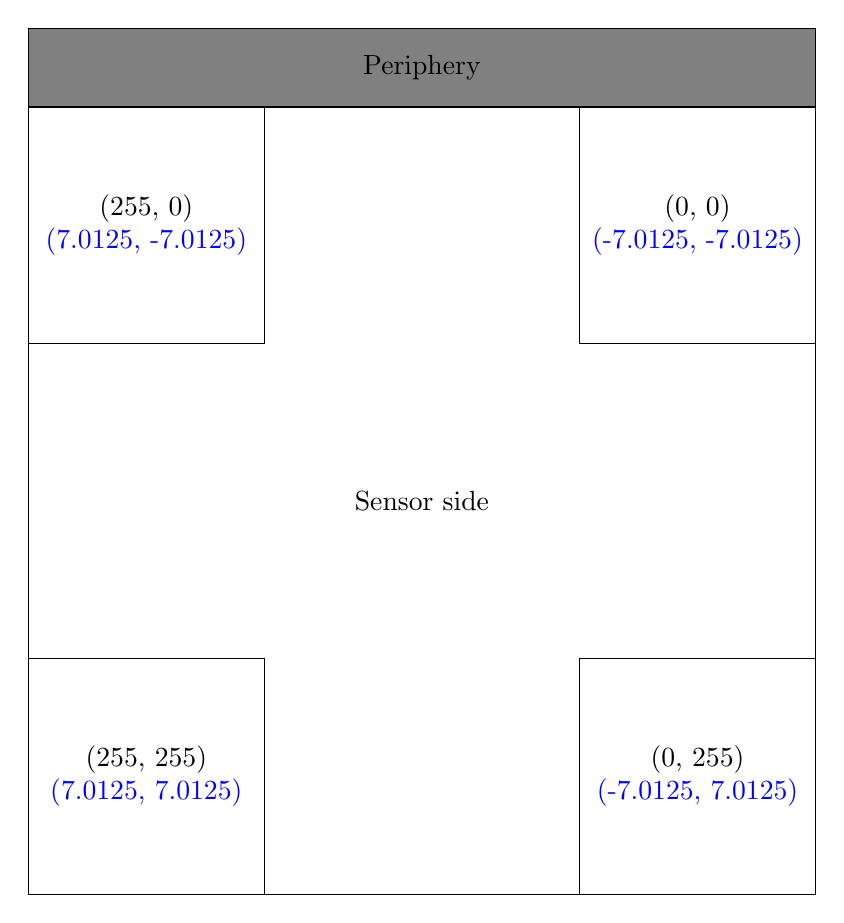
\begin{tikzpicture}
    \begin{scope} 

      \draw (0, 0) rectangle (10, 10) node[pos=.5] {Sensor side};
      \draw[fill=gray] (0, 10) rectangle (10, 11) node[pos=.5]
      {Periphery};

      \draw (0, 10) rectangle (3, 7) node[align=center, pos=.5] {(255, 0) \\ \textcolor{blue}{(7.0125, -7.0125)}};
      \draw (7, 10) rectangle (10, 7) node[align=center, pos=.5] {(0, 0) \\ \textcolor{blue}{(-7.0125, -7.0125)}};
      
      \draw (0, 0) rectangle (3, 3) node[align=center, pos=.5] {(255,
        255) \\ \textcolor{blue}{(7.0125, 7.0125)}};
      \draw (7, 0) rectangle (10, 3) node[align=center, pos=.5] {(0, 255) \\ \textcolor{blue}{(-7.0125, 7.0125)}};
      % \draw[help lines,xstep=.1,ystep=.1] (0, 0) grid (10,10);
      % \foreach \x in {0,1,...,9} { \node [anchor=north] at (\x/10,0) {0.\x}; }
      % \foreach \y in {0,1,...,9} { \node [anchor=east] at (0,\y/10)
      %   {0.\y}; }

    %   \draw[step=2cm,color=gray] (-5, -5) grid (5, 5);
    %   \matrix[matrix of nodes,nodes={inner sep=0pt,text width=2cm,align=center,minimum height=2cm}]{
    %     {(255, 0) \\ \textcolor{blue}{(7.0125, -7.0125)}} & &  & {(0,0) \\ \textcolor{blue}{(-7.0125, -7.0125)}} \\
    %     &  &  &  \\
    %     &  &  &  \\
    %     {(255, 255) \\ \textcolor{blue}{(7.0125, 7.0125)}} &  &  & {(0, 255) \\ \textcolor{blue}{(-7.0125, 7.0125)}} \\};
    \end{scope}  
  \end{tikzpicture}
  \caption{}
  \label{fig:coordinateSystem}
\end{figure}


\section{Timepix3 telescope resolution}
\label{sec:TelescopeResolution}


\subsection{Biased residuals on each telescope plane}

\subsubsection{Track vs. hit}
\subsubsection{Track vs. MC}
\subsubsection{Hit vs. MC}

\subsection{Unbiased resolution on the DUT}
\subsubsection{Track vs. hit}
\subsubsection{Track vs. MC}
\subsubsection{Hit vs. MC}